\chapter*{Mathematical Synthesis}
\addcontentsline{toc}{chapter}{Mathematical Synthesis}

Machine intelligence is built from a small number of recurring mathematical objects: data distributions, hypothesis classes, losses, optimization procedures, and uncertainty estimates. The course becomes easier to read when these are kept separate. Optimization asks whether we found a good parameter. Generalization asks whether that parameter will remain good away from the finite training sample.

\begin{figure}[h]
\centering
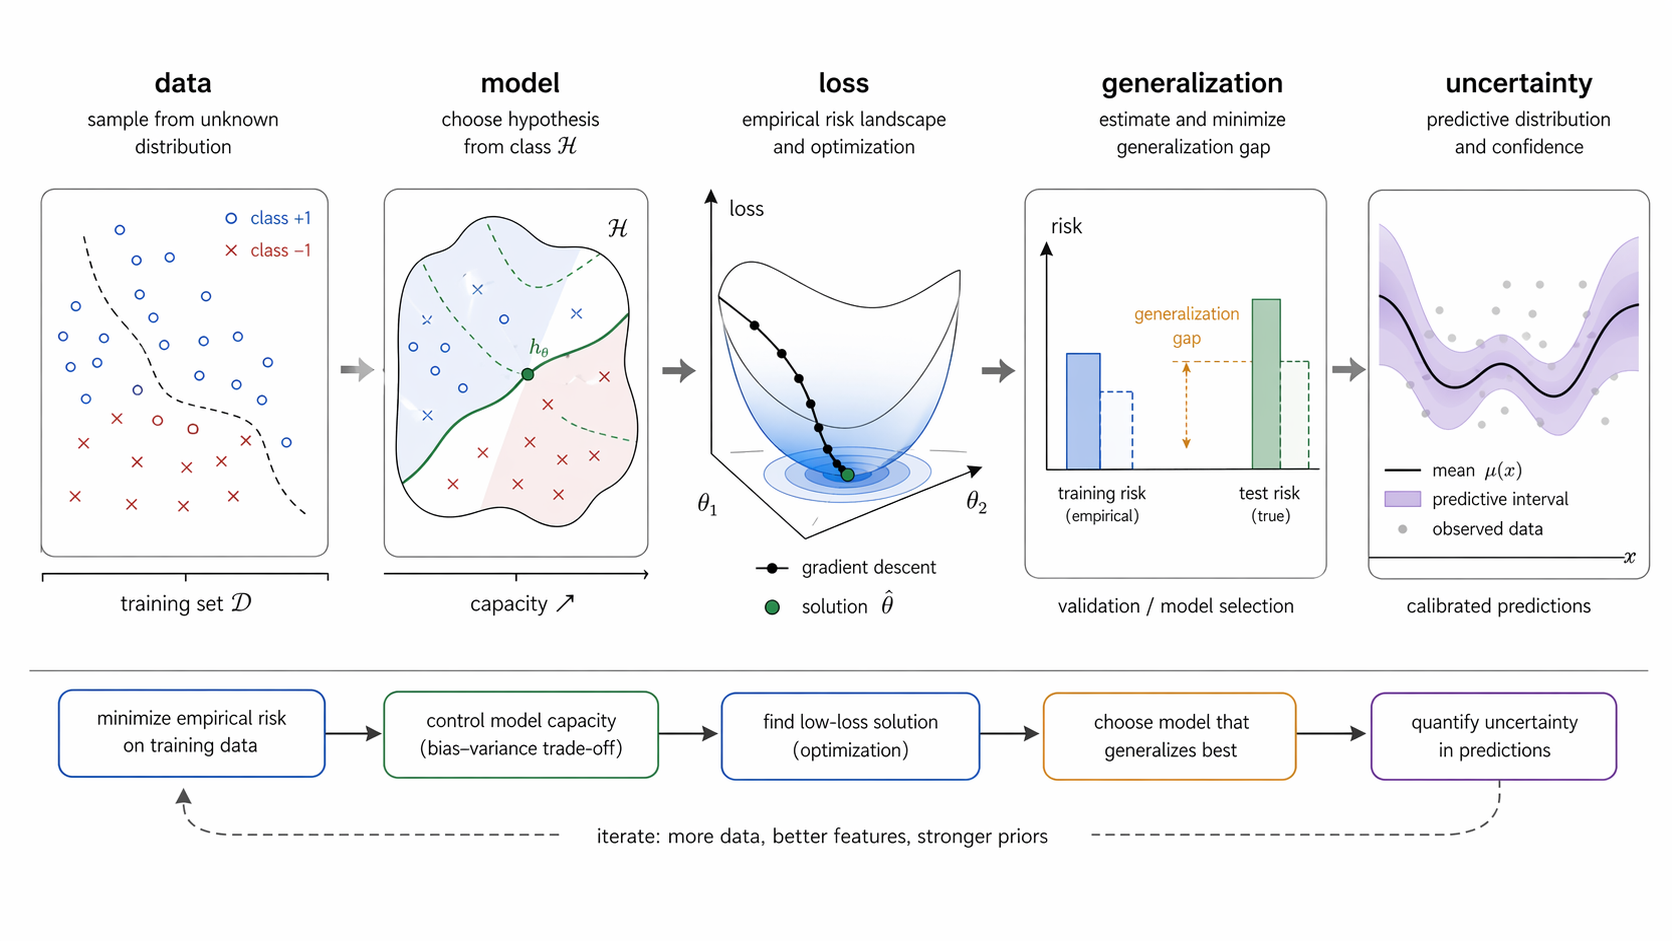
\includegraphics[width=0.96\textwidth]{figures/codex-mi1-risk-generalization.png}
\caption{The main loop of supervised learning. Data define an empirical problem, a model class restricts the functions we can choose, optimization searches the empirical-risk landscape, validation estimates generalization, and uncertainty describes what predictions should be trusted.}
\end{figure}

\section*{Empirical Risk Is Only A Proxy}

For a hypothesis \(h_\theta\) and loss \(\ell\), training minimizes
\[
  \widehat{R}_n(\theta)
  =
  \frac{1}{n}\sum_{i=1}^{n}
  \ell\bigl(h_\theta(x_i),y_i\bigr).
\]
The real object of interest is the population risk
\[
  R(\theta)
  =
  \E_{(X,Y)\sim P}
  \left[
    \ell\bigl(h_\theta(X),Y\bigr)
  \right].
\]
The empirical risk is computable; the population risk is what we actually care about. The gap between them is not a technical nuisance but the central difficulty of learning from data.

\begin{keyequation}[Learning problem]
\[
  \theta^\ast \in \argmin_\theta R(\theta),
  \qquad
  \hat{\theta}_n \in \argmin_\theta \widehat{R}_n(\theta).
\]
\tcblower
Learning succeeds when \(\widehat{R}_n\) is informative enough that \(\hat{\theta}_n\) also has small \(R\). This requires data, inductive bias, and an optimizer that finds a useful region of parameter space.
\end{keyequation}

\section*{Three Errors To Keep Apart}

A crisp way to diagnose a model is to separate the failure modes:
\[
  R(\hat{\theta})
  =
  \underbrace{R(\theta^\ast_{\mathcal{H}})}_{\text{approximation}}
  +
  \underbrace{R(\hat{\theta}_n)-R(\theta^\ast_{\mathcal{H}})}_{\text{estimation}}
  +
  \underbrace{R(\tilde{\theta})-R(\hat{\theta}_n)}_{\text{optimization, if any}}.
\]
The exact decomposition depends on notation, but the distinction is stable. Approximation error comes from the hypothesis class being too small or badly matched. Estimation error comes from finite data. Optimization error comes from failing to find a good empirical solution.

Deep learning often reduces approximation error by expanding the function class, then relies on architecture, data augmentation, regularization, and optimization bias to control the estimation problem.

\section*{Geometry Of Classification}

For a linear classifier,
\[
  h(x) = \sign(w^\top x + b),
\]
the decision boundary is the hyperplane \(w^\top x + b=0\). The vector \(w\) is normal to the boundary, so changing \(w\) rotates the separator and changing \(b\) translates it. Margin methods turn this geometry into an objective: choose a boundary that classifies the data while leaving a large buffer around it.

This geometric picture survives inside nonlinear models. A neural network first transforms \(x\) into a representation \(\phi_\theta(x)\), then makes a decision in that new coordinate system. The hard part is learning a representation in which the final decision boundary is simple.

\section*{Uncertainty Is Part Of The Output}

A point prediction says what the model thinks. A distribution says how strongly it thinks it. Bayesian inference makes this explicit:
\[
  p(\theta \mid D)
  =
  \frac{p(D\mid \theta)p(\theta)}{p(D)},
  \qquad
  p(y_\ast \mid x_\ast,D)
  =
  \int p(y_\ast\mid x_\ast,\theta)\,p(\theta\mid D)\,d\theta.
\]
Even when exact Bayesian inference is not used, this formula is the right mental model. Good machine-intelligence systems should distinguish uncertainty caused by noisy observations from uncertainty caused by missing data. Calibration, validation curves, and posterior or ensemble predictions are all attempts to keep that distinction visible.
